%%%%%%%%%%%%%%%%%%%%%%%%%%%%%%%%%%%%%%%%%
% Tufte Essay
% LaTeX Template
% Version 2.0 (19/1/19)
%
% This template originates from:
% http://www.LaTeXTemplates.com
%
% Authors:
% The Tufte-LaTeX Developers (https://www.ctan.org/pkg/tufte-latex)
% Vel (vel@LaTeXTemplates.com)
%
% License:
% Apache License, version 2.0
%
%%%%%%%%%%%%%%%%%%%%%%%%%%%%%%%%%%%%%%%%%

%----------------------------------------------------------------------------------------
%	PACKAGES AND OTHER DOCUMENT CONFIGURATIONS
%----------------------------------------------------------------------------------------

\documentclass[a4paper]{tufte-handout} % Use A4 paper by default, remove 'a4paper' for US letter

\usepackage{graphics}
\usepackage{graphicx} % Required for including images
\setkeys{Gin}{width=\linewidth, totalheight=\textheight, keepaspectratio} % Default images settings

\usepackage{amsmath, amsfonts, amssymb, amsthm} % For math equations, theorems, symbols, etc
%\usepackage{units} % Non-stacked fractions and better unit spacing
\usepackage{physics}
\usepackage{cancel}
\usepackage{siunitx}

\usepackage{booktabs} % Required for better horizontal rules in tables

% For newtcbtheorem
\usepackage[most]{tcolorbox}
\usepackage{cleveref}
\usepackage{fancybox}		% Recuadros emph eqn

\usepackage{empheq}			% Recuadros para ecuaciones

\setlength{\parskip}{1em}


%----------------------------------------------------------------------------------------
%	TITLE SECTION
%----------------------------------------------------------------------------------------

\title{Quantum Computation\\ Quantum Circuits Activity}

\author{Francisco Vazquez-Tavares}

\date{\today} % Date, use \date{} for no date


%----------------------------------------------------------------------------------------
%	COMMANDS SECTION
%----------------------------------------------------------------------------------------

\newcommand{\hata}{\hat{a}}
\newcommand{\hatad}{\hat{a}^\dagger}
\newcommand{\QDi}{\hat{X}_1}
\newcommand{\QDj}{\hat{X}_2}

\newtcbtheorem[]{prob}{Problem}%
    {enhanced,
    colback = black!5, %white,
    colbacktitle = black!5,
    coltitle = black,
    boxrule = 0pt,
    frame hidden,
    borderline west = {0.5mm}{0.0mm}{black},
    fonttitle = \bfseries\sffamily,
    breakable,
    before skip = 3ex,
    after skip = 3ex
}{def}

\bibliographystyle{apalike}
\nobibliography{}

%----------------------------------------------------------------------------------------

\begin{document}

\maketitle % Print the title section
\justifying

%----------------------------------------------------------------------------------------
%	ESSAY BODY
%----------------------------------------------------------------------------------------

\begin{prob}{~}{label1}
    Compare the effect of the following two circuits

    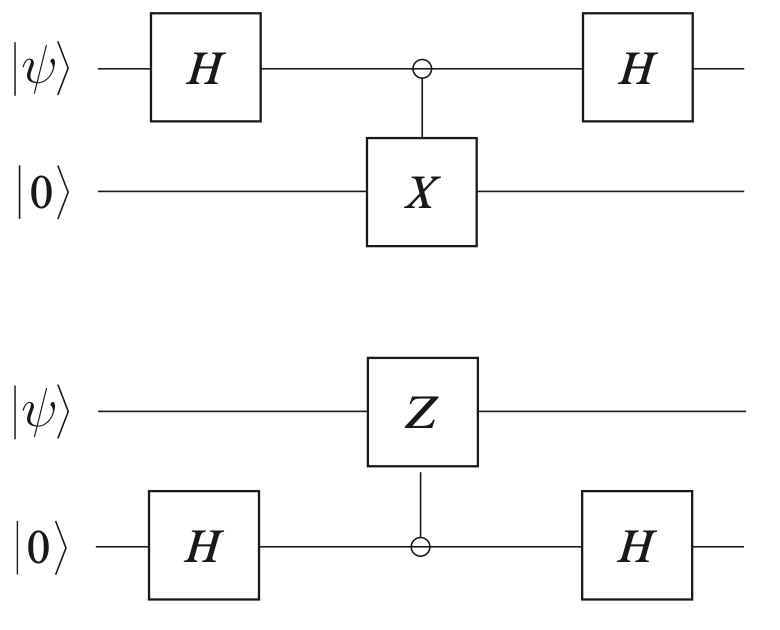
\includegraphics[width=0.9\textwidth]{imgs/image-7.png}

\end{prob}

Let's consider the following general state $\ket{\psi}=a\ket{0} + b\ket{1}$ with $a,c\in\mathbb{C}$.
The first circuit can be represented with the following algebraic expression
\begin{gather*}
    \left[\left(\hat{H}\otimes\mathbb{1}\right)\left(\Lambda\hat{X}\right)\left(\hat{H}\otimes\mathbb{1}\right)\right]\left(\ket{\psi}\otimes\ket{0}\right).
\end{gather*}
Where $\Lambda\hat{X}$ denotes the controlled $\hat{X}$ gate ($\dyad{0}\otimes\mathbb{1} + \dyad{1}\otimes\hat{X})$,
$\hat{H}$ is the Haddamard gate and $\hat{X}$ is the $X$ gate.

Starting with the first gate,
\begin{align*}
    \left(\hat{H}\otimes\mathbb{1}\right)\left(\ket{\psi}\otimes\ket{0}\right) &= \hat{H}\ket{\psi}\otimes\mathbb{1}\ket{0} \\
                                                                               &= \left[\frac{a}{\sqrt{2}}\qty(\ket{0}+\ket{1})+\frac{b}{\sqrt{2}}\qty(\ket{0}-\ket{1})\right]\otimes\mathbb{1}\ket{0} \\
                                                                               &= \left[\frac{\qty(a+b)}{\sqrt{2}}\ket{0}+\frac{\qty(a-b)}{\sqrt{2}}\ket{1}\right]\otimes\mathbb{1}\ket{0} \\
                                                                               &= \frac{\qty(a+b)}{\sqrt{2}}\ket{00}+\frac{\qty(a-b)}{\sqrt{2}}\ket{10}.
\end{align*}

Now we compute the controlled $\hat{X}$ gate with the new state with the following mnemonic rule, \textit{It flips the second qubit if the first qubit is \num{1} and leaves unchanged otherwise}, therefore
\begin{gather*}
    \Lambda\hat{X}\left[\frac{\qty(a+b)}{\sqrt{2}}\ket{00}+\frac{\qty(a-b)}{\sqrt{2}}\ket{10}\right] = \frac{\qty(a+b)}{\sqrt{2}}\ket{00}+\frac{\qty(a-b)}{\sqrt{2}}\ket{11}=\ket{\psi_2}.
\end{gather*}

Finally, we apply the last Haddamard gate into the nwe state,
\begin{align*}
    \left(\hat{H}\otimes\mathbb{1}\right)\ket{\psi_2} &=\frac{\qty(a+b)}{\sqrt{2}}\hat{H}\ket{0}\otimes\mathbb{1}\ket{0} + \frac{\qty(a-b)}{\sqrt{2}}\hat{H}\ket{1}\otimes\mathbb{1}\ket{1} \\
                                                      &=\frac{\qty(a+b)}{\sqrt{2}}\left(\frac{1}{\sqrt{2}}\qty(\ket{0}+\ket{1})\right)\otimes\mathbb{1}\ket{0} + \frac{\qty(a-b)}{\sqrt{2}}\left(\frac{1}{\sqrt{2}}\qty(\ket{0}-\ket{1})\right)\otimes\mathbb{1}\ket{1} \\
                                                      &=\frac{\qty(a+b)}{2}\left(\ket{00}+\ket{10}\right) + \frac{\qty(a-b)}{2}\left(\ket{01}-\ket{11}\right).
\end{align*}
After expanding the expression and minor algebraic manipulations we can express the final state in terms of the of the Bell states,
\begin{gather*}
    \left(\hat{H}\otimes\mathbb{1}\right)\ket{\psi_2}=\frac{a}{\sqrt{2}}\left(\ket{\Psi^+} + \ket{\Phi^+} \right) + \frac{b}{\sqrt{2}}\left(\ket{\Psi^+} - \ket{\Phi^-} \right)
\end{gather*}

Bottom circuit.

\begin{align*}
    \left[\left(\mathbb{1}\otimes\hat{H}\right)\left(\Lambda\hat{Z}\right)\left(\mathbb{1}\otimes\hat{H}\right)\right]\left(\ket{\psi}\otimes\ket{0}\right)
\end{align*}



\begin{prob}{~}{label2}
    Show that the following quantum circuit is equivalent to a controlled Z-gate

    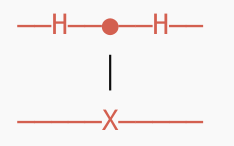
\includegraphics[width=0.9\textwidth]{imgs/image-8.png}

\end{prob}


\begin{prob}{~}{label3}
    The three qubit GHZ-state is defined as\[\ket{GHZ}=\frac{1}{2}\left(\ket{000}+\ket{111}\right).\]

    Design a circuit that upon of the separable state $\ket{000}$ constructs the GHZ-state.

\end{prob}



\begin{comment}
The expectation value of an operator (or quantum gate) $A$ over a qubit $\ket{\psi}$ is defined as
\begin{equation}
    \expval{A} = \expval{A}{\psi}.
\end{equation}
Consider the general state
\begin{equation}
    \ket{\psi} = a\ket{0} + b\ket{1},\quad a,b\in\mathbb{C},
\end{equation}
and define the map
\begin{equation}
    \ket{\psi} \mapsto\hat{n} = \left(\expval{X},\expval{Y},\expval{Z}\right).
\end{equation}

\begin{prob}{~}{label1}

    Show that the entries of the vector $\hat{n}$ fulfill
    \begin{align*}
        n_x &= \expval{X} = 2\Re(\bar{a}b) \\
        n_y &= \expval{Y} = 2\Im(\bar{a}b) \\
        n_z &= \expval{Z} = \abs{a}^2 - \abs{b}^2.
    \end{align*}
    and its norm is equal to \num{1}.
    The overline $\bar{x}$ stands for the complex conjugate of $x$.
    You might work with the conventional matrix representation.

\end{prob}

Let's start with $n_x$,
\begin{align*}
    n_x &= \expval{X}{\psi} = \mqty(\bar{a} & \bar{b})\mqty(\pmat{1})\mqty(a \\ b) \\
        &= \mqty(\bar{a} & \bar{b})\mqty(b \\ a) \\ 
        &= \bar{a}b + \bar{b}a.
\end{align*}
Recalling that $\Re(z)=(z+\bar{z})/2$, we can re-write,
\begin{align*}
    n_x = 2\Re(\bar{a}b).
\end{align*}

Moving forward to $n_y$ we repeat the same process,
\begin{align*}
    n_y &= \expval{Y}{\psi} = \mqty(\bar{a} & \bar{b})\mqty(\pmat{2})\mqty(a \\ b) \\
        &= \mqty(\bar{a} & \bar{b})\mqty(ib \\ -ia) \\ 
        &= i\left(\bar{a}b - \bar{b}a\right).
\end{align*}
Recalling that $\Im(z)=(z-\bar{z})/2$, we can re-write,
\begin{align*}
    n_y = 2\Im(\bar{a}b).
\end{align*}

Finally, for $n_z$, we repeat one last time,
\begin{align*}
    n_z &= \expval{Z}{\psi} = \mqty(\bar{a} & \bar{b})\mqty(\pmat{3})\mqty(a \\ b) \\
        &= \mqty(\bar{a} & \bar{b})\mqty(a \\ -b) \\ 
        &= \abs{a}^2 - \abs{b}^2.
\end{align*}

Now, to compute the norm we need to sum the squared of the components and take the squared of the result.
Let's start by computing the squared of each component,
\begin{align*}
    n_x^2 &= \left(\bar{a}b + \bar{b}a\right)^2 = \bar{a}^2b^2 + 2\abs{a}^2\abs{b}^2 + \bar{b}^2a^2 \\
    n_y^2 &= \left(i\left(\bar{a}b - \bar{b}a\right)\right)^2 = -\bar{a}^2b^2 + 2\abs{a}^2\abs{b}^2 - \bar{b}^2a^2 \\
    n_z^2 &= \left(\abs{a}^2 - \abs{b}^2\right)^2 = \abs{a}^4 - 2\abs{a}^2\abs{b}^2 + \abs{b}^4.
\end{align*}
Now, we add the terms,
\begin{align*}
    n_x^2 + n_y^2 + n_z^2 &= \abs{a}^4 + 2\abs{a}^2\abs{b}^2 + \abs{b}^4. 
\end{align*}
The nex step is to assume that the state $\ket{\psi}$ is normalize, such that $\ip{\psi}{\psi}=1=\abs{a}^2+\abs{b}^2$.
We can derive the following identities, $\abs{a}^2=1-\abs{b}^2$ and  $\abs{a}^4=1-2\abs{b}^2+\abs{b}^4$.
\begin{align*}
    n_x^2 + n_y^2 + n_z^2 &= 1 - 2\abs{b}^2 + \abs{b}^4 + 
                            2\abs{b}^2 - 2\abs{b}^4 + \abs{b}^4 \\
                          &= 1.
\end{align*}
Hence the norm of $\hat{n}$ is \num{1}.


\begin{prob}{~}{label2}
    The qubit $\ket{\psi}$ can be parametrized in the following way,
    \begin{equation}
        \ket{\psi} = \cos\left(\frac{\theta}{2}\right)\ket{0} + e^{i\varphi}\sin\left(\frac{\theta}{2}\right)\ket{1},
    \end{equation}
    with $\theta\in[0,\pi/2],\quad\varphi\in[1,2\pi].$
    Using the results obtained in the previous part prove that the components of $\hat{n}$ are the usual spherical coordinates,
    \begin{align*}
        n_x &= \sin\theta\cos\varphi \\
        n_y &= \sin\theta\sin\varphi \\
        n_z &= \cos\theta.
    \end{align*}
    This procedure justifies why an arbitrary qubit is identified with a point in the Bloch sphere, which is also called the qubit projective space.
\end{prob}

\marginpar{
Usefull trigonometric and complex exponentials identities for the excersices.
\begin{gather*}
    \cos(A)\sin(B) = \frac{\sin(A+B)-\sin(A-B)}{2} \\
    \cos(x) = \frac{1}{2}\left(e^{ix}+e^{-ix}\right) \\
    \sin(x) = \frac{1}{2i}\left(e^{ix}-e^{-ix}\right)
\end{gather*}
}

We can identify that $a=\cos\qty(\theta/2)$ and $b=e^{i\varphi}\sin\qty(\theta/2)$, hence,
\begin{align*}
    n_x &= \bar{a}b + \bar{b}a \\
        &= \left(e^{i\varphi}+e^{-i\varphi}\right)\cos\left(\frac{\theta}{2}\right)\sin\left(\frac{\theta}{2}\right) \\
        &= 2\cos\left(\varphi\right)\frac{1}{2}\sin\left(\theta\right)\\
        &= \cos\varphi\sin\theta.
\end{align*}
Moving on to the next component,
\begin{align*}
    n_y &= \bar{a}b - \bar{b}a \\
        &= \left(e^{i\varphi} - e^{-i\varphi}\right)\cos\left(\frac{\theta}{2}\right)\sin\left(\frac{\theta}{2}\right) \\
        &= 2\sin\left(\varphi\right)\frac{1}{2}\sin\left(\theta\right)\\
        &= \sin\varphi\sin\theta.
\end{align*}
Finally,
\begin{align*}
    n_z &= \abs{a}^2 - \abs{b}^2 \\
        &= \cos^2\left(\frac{\theta}{2}\right) - \sin^2\left(\frac{\theta}{2}\right) \\
        &= \cos\left(\theta\right).
\end{align*}
\end{comment}

\end{document}
